\documentclass{beamer}

\usepackage[utf8]{inputenc}
\usepackage[T1]{fontenc}
\usepackage{multicol}
\usepackage{tikz}
\usepackage{xcolor}
\usepackage{listings}


\usetikzlibrary{decorations.pathmorphing,patterns}

\title{TP 11 : Loi de Hooke}
\author{Cédrick, Raphaël J, Romain}

\beamertemplatenavigationsymbolsempty

\lstdefinestyle{algo}{
	mathescape=true,
	extendedchars=true,
	showstringspaces=false,
	tabsize=6,
	breaklines=true,
	framexleftmargin=0mm,
	frame={L},
	frameround=tt,
	numbers=left,
	%captionpos=t,
	%linewidth=0.8\textwidth,
	xleftmargin=.2\textwidth, xrightmargin=.2\textwidth,
	emph={Alors, AutreSi, FinPour, FinSi, FinTantQue, Pour, Retourner, Si, Sinon, TantQue},
	emphstyle=\bf,
	commentstyle=\color{gray},
	columns=flexible,
basicstyle=\ttfamily,}
\newcommand{\lil}{\lstinline[style=algo]}

\definecolor{vert}{RGB}{50, 168, 82} % Définir une couleur personnalisée
\definecolor{rouge}{RGB}{150, 11, 11} % Définir une couleur personnalisée

\date{}

\begin{document}

\frame{\titlepage}

\begin{frame}
    \frametitle{Sommaire}
    \tableofcontents
\end{frame}

\section{I Formule de Hooke}

\begin{frame}

    \frametitle{I Formule de Hooke}

    \subsection{I.1 À tout instant}
    \framesubtitle{I.1 À tout instant}

        \begin{columns}
            \begin{column}{0.75\textwidth}
            D'après la \textit{\textbf{Loi de Hooke}}, $$ \boxed{\forall t, \quad \overrightarrow{F_{\text{élastique}}} =  -k \times (l(t) - l_{0}) \overrightarrow{u_{ext}}}  $$
            avec :
            $\begin{cases} 
                k \text{ la constante de raideur du ressort} \\ 
                l_{0}  \text{ la longueur à vide du ressort} \\
                l(t) \text{ la longueur instantanée du ressort}
            \end{cases}$
            \end{column}

            \begin{column}{0.25\textwidth}
                \begin{tikzpicture}[>=stealth, thick, font=\tiny]
                    % axe vertical descendants
                    \draw[->] (-0.25,-2) -> (-0.25,-7.5) node[below right]{$z$};

                    % vecteur unitaire orienté vers le bas
                    \draw[->,blue] (-0.25,-2) -> (-0.25,-2.5) node[midway, left]{$\overrightarrow{u_{ext}}$};
                    \node at (-0.25,-1.8){$O$};
                
                    % Support
                    \draw (-1.5,-2) -- (1,-2);
                
                    % Ressort chargé
                    \draw[decorate, decoration={coil, segment length=5pt, amplitude=3pt}] (0.5,-2) -- (0.5,-5) node[pos=-0.125]{\shortstack{Ressort \\ chargé}};
                    
                    % Ressort à vide.
                    \draw[decorate, decoration={coil, segment length=2.5pt, amplitude=3pt}] (-1,-2) -- (-1,-3.5) node[pos=-0.25]{\shortstack{Ressort \\ à vide}};
                    % Masse
                        \filldraw (0.5,-5.0) circle (0.1) node[below, right]{$M(m)$};
                    % Force élastique
                    \draw[->,vert] (0.5,-5) -- (0.5,-4.5) node[above, right]{$\overrightarrow{F_{\text{élastique}}}$};
                    % Poids
                    \draw[->,rouge] (0.5,-5) -- (0.5,-5.75) node[above, right]{$\overrightarrow{P}$};

                    %longueur l0
                    \draw[<->,thin] (-1.25,-2) -- (-1.25,-3.5) node[midway, left]{$l_{0}$};

                    %longueur l(t)
                    \draw[<->,thin] (0.25,-2) -- (0.25,-5) node[midway, left]{$l(t)$};
                    
                
                    
                \end{tikzpicture}
            \end{column}
        \end{columns}
        

\end{frame}

\begin{frame}

    \frametitle{I Formule de Hooke}

    \subsection{I.2 À l'équilibre}
    \framesubtitle{I.2 À l'équilibre}

    \begin{columns}
        \begin{column}{0.75\textwidth}
        \textit{\textbf{À l'équilibre}}, on a le principe fondamental de la dynamique suivant :
        \begin{align*}
            &\overrightarrow{P} + \overrightarrow{F_{\textit{élastique}}} = \overrightarrow{0} \\
            \intertext{En projetant selon $(Oz)$, on obtient :}
            &mg = k(l_{eq}-l_{0}) \\
            \implies & \boxed{m = \frac{k}{g} \cdot x}
        \end{align*}

        $\text{avec : } \boxed{x = l_{eq} - l_{0}} \text{ l'allongement du ressort chargé}$
        \end{column}

        \begin{column}{0.25\textwidth}
            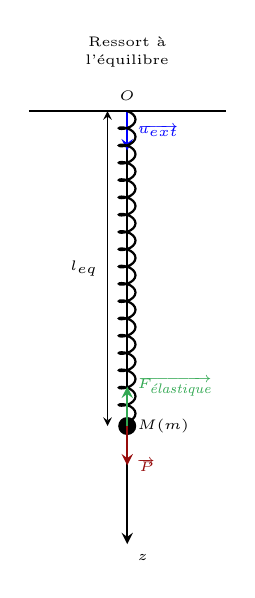
\begin{tikzpicture}[>=stealth, thick, font=\tiny]
                % axe vertical descendants
                \draw[->] (-0.25,-2) -> (-0.25,-7.5) node[below right]{$z$};

                % vecteur unitaire orienté vers le bas
                \draw[->,blue] (-0.25,-2) -> (-0.25,-2.5) node[midway, right]{$\overrightarrow{u_{ext}}$};
                \node at (-0.25,-1.8){$O$};
            
                % Support
                \draw (-1.5,-2) -- (1,-2);
            
                % Ressort
                \draw[decorate, decoration={coil, segment length=6.25pt, amplitude=3pt}] (-0.25,-2) -- (-0.25,-6) node[pos=-0.1875]{\shortstack{Ressort à \\ l'équilibre}};

                % Masse
                    \filldraw (-0.25,-6) circle (0.1) node[below, right]{$M(m)$};

                % Force élastique
                \draw[->,vert] (-0.25,-6) -- (-0.25,-5.5) node[above, right]{$\overrightarrow{F_{\textit{élastique}}}$};

                % Poids
                \draw[->,rouge] (-0.25,-6) -- (-0.25,-6.5) node[above, right]{$\overrightarrow{P}$};

                %longueur l_eq
                \draw[<->,thin] (-0.5,-2) -- (-0.5,-6) node[midway, left]{$l_{eq}$};
                
            
                
            \end{tikzpicture}
        \end{column}
    \end{columns}

\end{frame}

\section{II Déterminer k}

\begin{frame}

    \frametitle{II Déterminer k}

    \subsection{II.1 Par régression linéaire (étude à l'équilibre)}
    \framesubtitle{II.1 Par régression linéaire (étude à l'équilibre)}

        \begin{columns}
            \begin{column}{0.5\textwidth}
                \begin{figure}
                    \boxed{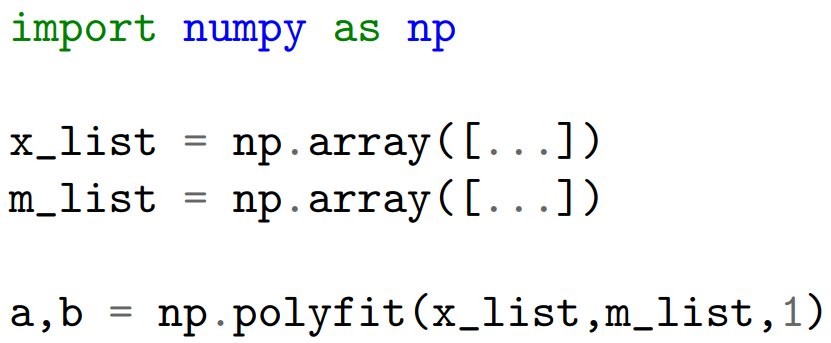
\includegraphics[width=\linewidth]{code.png}}
                    \parbox[b]{\linewidth}{\centering \tiny Figure 1 : Code essentiel à la régression}
                \end{figure}

                \begin{figure}
                    $$\boxed{m = \underbrace{\frac{k}{g}}_{\text{\lil{a}}} x + \underbrace{0}_{\text{\lil{b}}}}$$
                    \parbox[b]{\linewidth}{\centering \tiny Figure 2 : Relation entre formule et code}
                \end{figure}
            \end{column}
            \begin{column}{0.5\textwidth}
                \begin{figure}
                    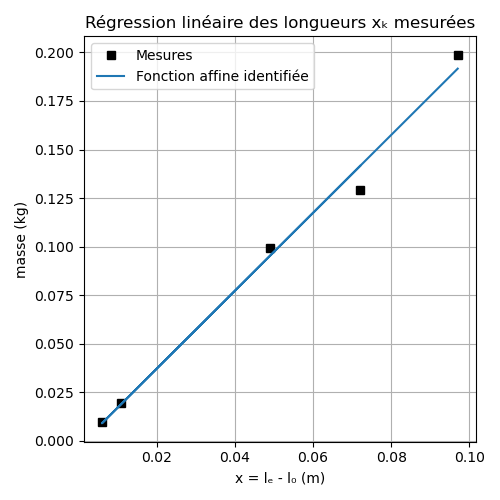
\includegraphics[width=\linewidth]{reglin.png}
                    \parbox[b]{\linewidth}{\centering \tiny Figure 3 : Régression linéaire de $m = ax + b$}
                \end{figure}
            \end{column}
        \end{columns}
\end{frame}

\begin{frame}
    \frametitle{II Déterminer k}

    \subsection{II.2 Par étude périodique (étude du mouvement)}
    \framesubtitle{II.2 Par étude périodique (étude du mouvement)}

    \begin{columns}
        \begin{column}{0.5\textwidth}
            \footnotesize 
            \begin{align*}
                \intertext{Principe fondamental de la dynamique :}
                &m \overrightarrow{a(M/R)} = m \overrightarrow{g} + \overrightarrow{F_{\textit{élastique}}} 
                \intertext{En projetant selon $(Oz)$  :}
                &m \ddot{z}(t) = mg -k(z(t)-l_{0})\\
                \implies & \ddot{z}(t) + \frac{k}{m}z(t) = g + \frac{kl_{0}}{m} \\
                \implies & \boxed{\ddot{z}(t) + \omega_{0}^{2}z(t) = g + \frac{kl_{0}}{m}} \\ \\
                \text{$\omega_{0}$ vérifie }&\text{alors : }
                \begin{cases}
                    \omega_{0} = \sqrt{\frac{k}{m}} \\ \\
                    \omega_{0} = \frac{2\pi}{T}
                \end{cases}
            \end{align*}
            
        \end{column}
        \begin{column}{0.5\textwidth}
            \footnotesize
            \begin{align*}
                \text{On a donc : }&\sqrt{k} = \frac{2\pi\sqrt{m}}{T} \\
                \implies &\boxed{k = \frac{4\pi^{2}m}{T^{2}}}
            \end{align*}
            \begin{figure}
                \boxed{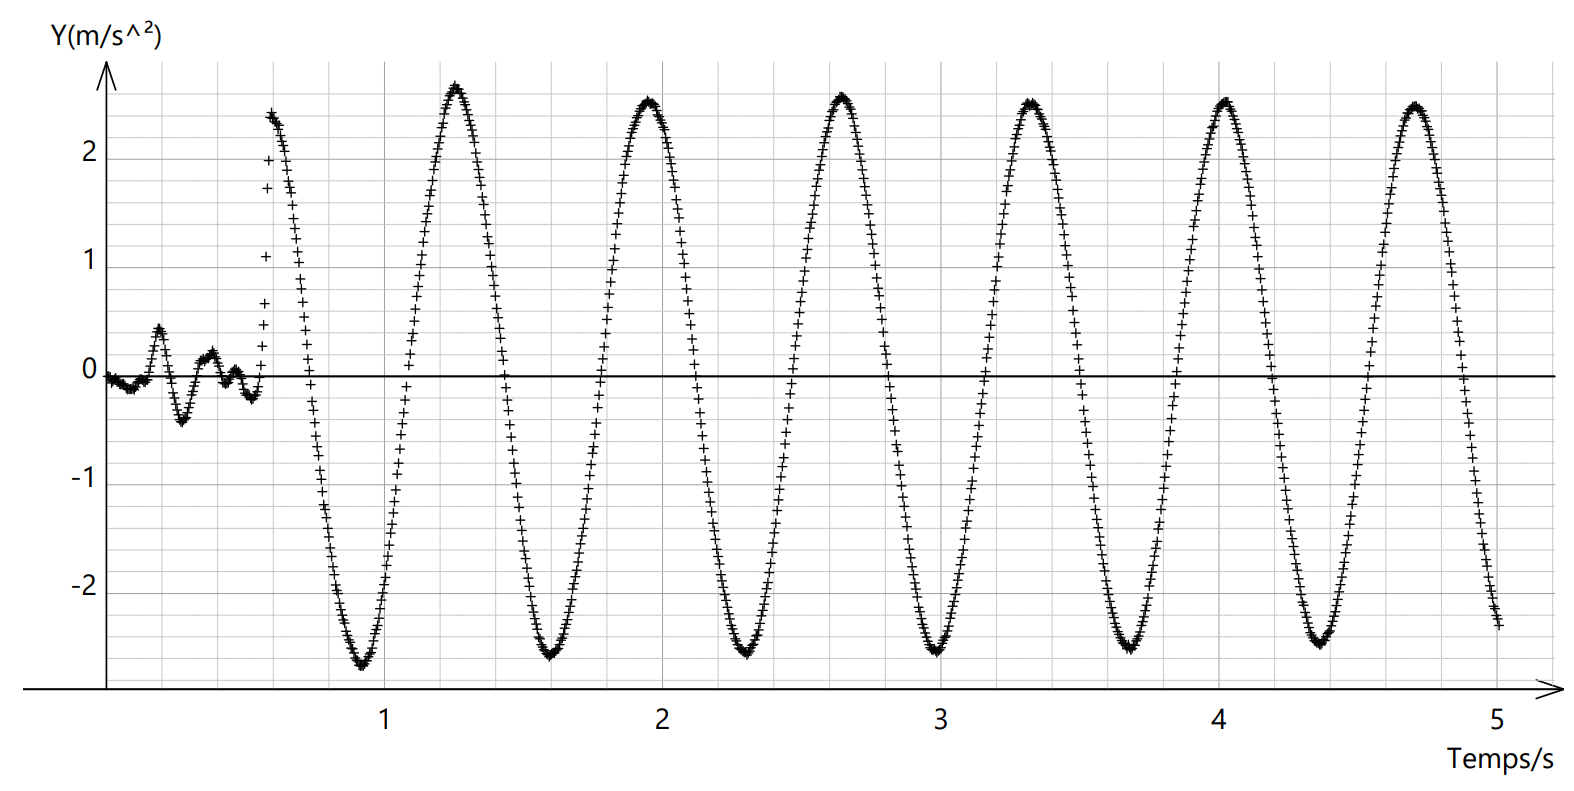
\includegraphics[width=\linewidth]{courbe z(t).png}}
                \parbox[b]{\linewidth}{\centering \tiny Figure 4 : Courbe de l'accélération verticale en fonction du temps}
            \end{figure}
        \end{column}
    \end{columns}



\end{frame}

\end{document}
